\section{Интеграция платформы на примере реального проекта}

\subsection{Введение}

Как уже упоминалось ранее, интерес к вопросам автоматизации и расширения программного обеспечения был вызван необходимостью интегрировать в новую версию коммерческого программного продукта поддержку данных возможностей. В старой версии продукта для этих целей использовалась {\it VBA}. При разработке новой версии была попытка использовать технологию {\it VSTA}, но она не увенчалась успехом (подробности были описаны в разделе~\ref{sec:use_exis_techn}).

Новая разработанная платформа для внедрения возможностей автоматизации и расширения изначально была протестирована на различных тестовых проектах. Это позволило оценить её эффективность, выявить и исправить ошибки, а также сравнить процесс интеграции разработанной платформы с существующими аналогами. Когда этап тестирования был завершён, а целесообразность использования новой разработки подтверждена, необходимо было внедрить платформу в реальное коммерческое приложение. 

В данной главе будет вкратце описано хост-приложение, в которое будет интегрирована платформа. Затем будут рассмотрены основные шаги интеграции. И в заключение будут подведены итоги и упомянуты преимущества и недостатки, выявленные при внедрении, в сравнении с существующими разработками.

\subsection{Описание подхода к интеграции}

На момент интеграции разработанной платформы работа над очередной версией проекта была практически завершена. За счёт этого в процессе интеграции должно было проявиться одно из основных преимуществ разработанной платформы перед существующими аналогами --- простота и удобство внедрения. На практике это должно означать, что:
\begin{itemize}
 \item при интеграции общая архитектура системы на должна претерпеть существенных изменений;
 \item необходимы лишь минимальные знания об области, в которой данное приложение решает задачи;
 \item детали реализации большинства подсистем не важны и могут быть неизвестны.
\end{itemize}

Исходя из этих принципов, и будет описываться коммерческое приложение.

\subsection{Описание приложения.}

{\it ITM (Integrated Treasury Manager)} --- программный продукт для работы с инвестиционными портфелями. 

Главное окно приложения показано на рисунке~\ref{pic:itm-main-wnd}.
\begin{figure}[!h]
    \centering
    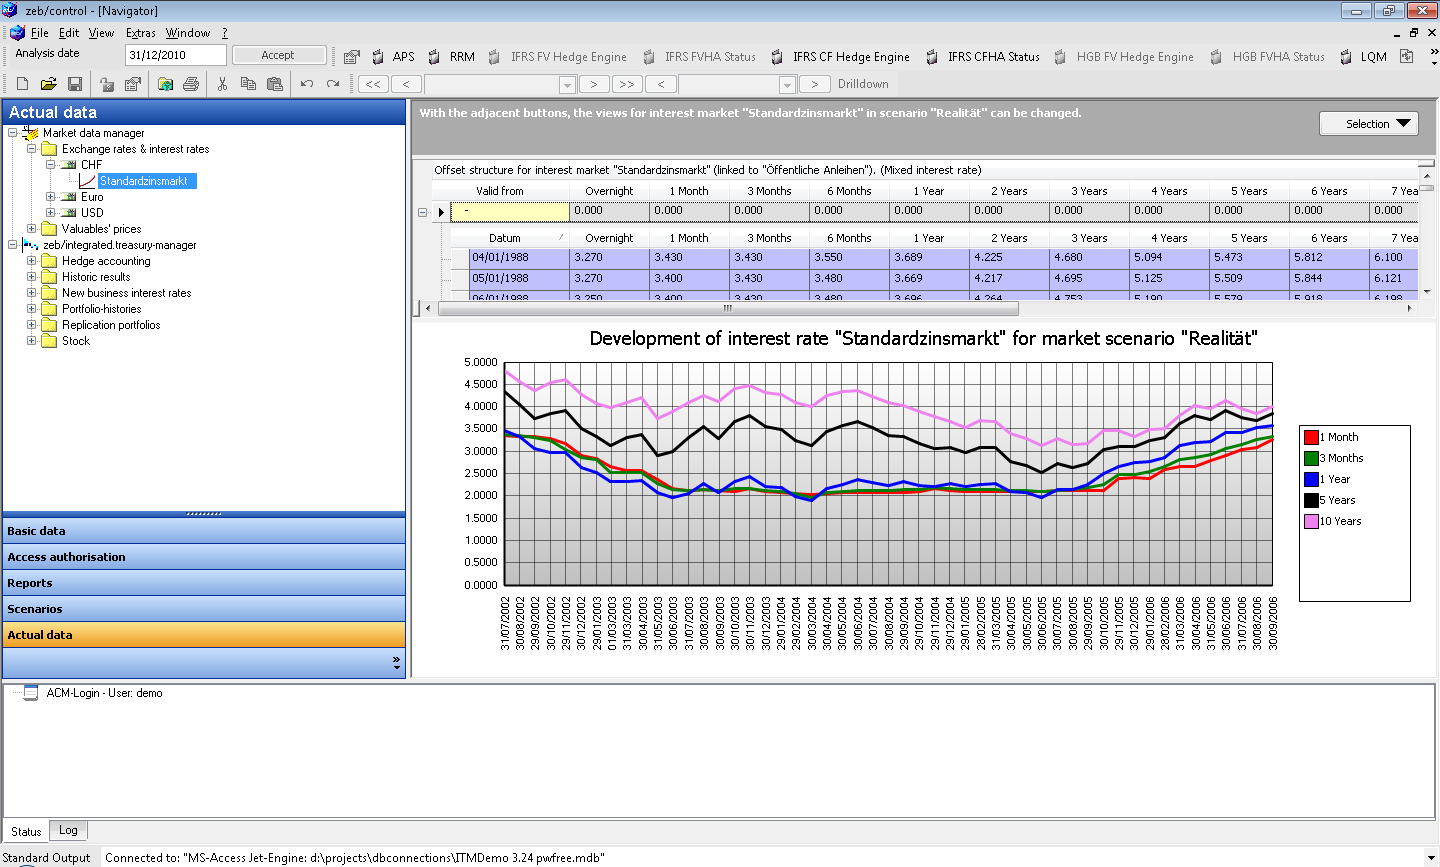
\includegraphics[width=16cm]{itm-main-wnd.png}
    \caption{Главное окно приложения ITM}
    \label{pic:itm-main-wnd}
\end{figure}

Рассматривая структуру этого приложения, можно выделить несколько основных модулей:
\begin{enumerate}
 \item модуль для работы с данными (информация о курсах валют, ценных бумагах, клиентах...);
 \item модуль, содержащий набор функций и алгоритмов, специфичных для предметной области;
 \item модуль, осуществляющий симуляцию различных процессов, специфичных для предметной области;
 \item модуль для генерации отчётов.
\end{enumerate}

С точки зрения дизайна, можно выделить несколько основных сущностей проекта:
\begin{itemize}
 \item графический интерфейс пользователя; 
 \item набор сервисов;
 \item набор объектов бизнес-логики.
\end{itemize}

Графический интерфейс (GUI, graphical user interface) приложения довольно сложный, включает в себя множество диалоговых окон (в том числе динамически создающихся), компонентов для отображения графиков и таблиц, панелей управления, элементов меню. При построении графического интерфейса и его связи с бизнес-логикой использовались различные подходы и шаблоны проектирования~\cite{band-four}. Один из сервисов приложения (см. ниже) предоставляет возможность пользовательскому коду динамически добавлять или изменять некоторые элементы GUI, максимально абстрагируясь деталей реализации графического интерфейса. Эта особенность будет использована при интеграции платформы в ITM.

Под сервисами приложения понимается набор алгоритмов, методов и структур данных, реализованных в ITM. Чаще всего для этих целей используется шаблон проектирования {\it Singleton}~\cite{band-four}. Сервисы могут быть использованы как внутри приложения, так и пользовательским кодом, написанном для автоматизации или расширения. Эти возможности будут также активно использованы при интеграции разработанной платформы в ITM.

Набор объектов бизнес-логики --- это множество классов, имитирующих объекты предметной области (банкинг, финансы, инвестии\dots). Такие объекты доступны из пользовательского кода, в котором могут быть созданы непосредственно, либо получены в качестве результата при выполнении какого-либо сервиса.

\subsection{Интеграция}

Для обеспечения возможностей взаимодействия с платформой в приложение внедряется новый модуль --- {\it APC (Application Programming Components)}. На схеме, представленной на рисунке~\ref{fw_arch1} из раздела~\ref{sec:fw_arch}, этот модуль называется <<модуль поддержки расширений>>. {\it APC} --- единственный модуль, добавление которого связано непосредственно с модификацией исходного кода приложения. В этом заключается одно из преимуществ разработанной платформы, отсутствующие в существующих продуктах.

На рисунке~\ref{pic:itm-integration} показана схема взаимодействия основного приложения (ITM) и платформы для автоматизации и расширения. Описание технологий, использующихся для взаимодействия тех или иных модулей, было приведено ранее, поэтому здесь нет смысла останавливаться на этом подробнее.

\begin{figure}[!h]
    \centering
    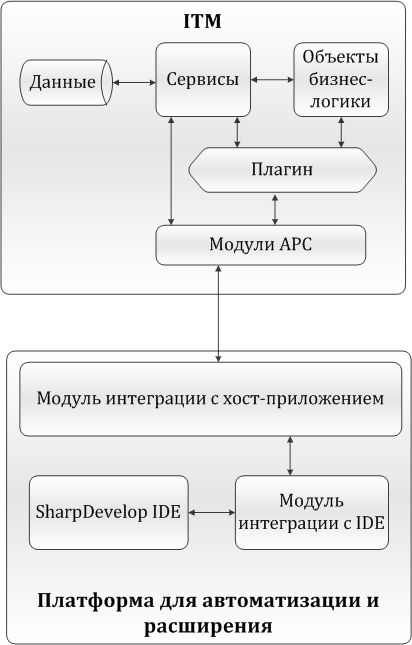
\includegraphics[width=9cm]{itm-integration.png}
    \caption{Схема взаимодействия ITM и платформы для автоматизации и расширения}
    \label{pic:itm-integration}
\end{figure}

Как видно из схемы, плагин (то есть пользовательское расширение или макрос) взаимодействует непосредственно с сервисами приложения и объектами бизнес-логики. Детали этого взаимодействия могут отличаться в зависимости от конкретной ситуации и требований к безопасности. В некоторых случаях могут потребоваться прокси-объекты. Но в целом это не меняет подхода к интеграции.

Модуль {\it APC} на стороне хост-приложения является точкой сочленения ITM и платформы для автоматизации и расширения. {\it APC} напрямую взаимодействует с сервисами приложения для обеспечения тесной интеграции. {\it APC} в некотором смысле является фасадом~\cite{band-four} и позволяет расширению взаимодействовать с компонентами основного приложения, не вдаваясь в детали реализации. Помимо этого модули {\it APC} предоставляют интерфейс для управления расширениями и средой разработки, а также позволяют хост-приложению реагировать на события IDE.

Взаимодействие компонентов внутри платформы для интеграции и расширения подробно описывалось ранее. Платформа не претерпевает никаких изменений при интеграции в ITM, поэтому детально останавливаться на этом здесь не имеет смысла.

\subsection{Выводы}

При интеграции разработанной платформы в приложение ITM, работа над очередной версией которого была практически завершена, проявилось одно из основных преимуществ платформы перед существующими аналогами. Интеграция действительно была проста, а изменения в архитектуре (и исходном коде) хост-приложения --- минимальны. Платформа довольно гармонично вписалась в общий дизайн приложения, несмотря на то, что при проектировании ITM практически никак не учитывалась специфика платформы. 

Интеграция платформы на примере реального коммерческого проекта также показала, что эта разработка даёт хорошие результаты не только при её тестировании на демонстрационных проектах, имеющих небольшой размер и зачастую не позволяющих полностью оценить возможности платформы, но и в крупных программных комплексах.

Как упоминалось ранее, в ITM изначально внедрялась {\it VSTA}, но эта попытка не увенчалась успехом. Невозможно <<количественно>> оценить сложность интеграции той или иной разработки в программный продукт, однако по субъективному мнению разработчиков интеграция {\it VSTA} сопровождалось большим числом проблем и потребовала большего времени.

Таким образом можно сделать вывод о том, что разработанная платформа действительно пригодна для использования в крупных проектах. Она решает поставленные задачи и предоставляет разработчикам мощный инструмент для добавления возможностей автоматизации и расширения в программное обеспечение. Более подробные выводы, а также сравнение с аналогичными разработками, будет приведено ниже, в главе~\ref{sec:analogs-comparison}.

\pagebreak